\documentclass{article}
\usepackage[utf8]{inputenc}
\usepackage{amssymb, amsmath,hyperref,verbatim,listings,graphicx,subfigure,fullpage}

\begin{document}

\title{UML computer project 2}
\author{
Juha-Antti Isojärvi\\
013455341 \\
Department of Mathematics and Statistics\\
Master student
\and
Mikko Sysikaski\\
013573016\\
Department of Computer Science\\
Master student}
\date{}
\maketitle

\section{Exercise set 2}
\subsection{Exercise 1}
Sample covariance and mean:
\begin{verbatim}
> mean(y1)
[1] -0.007008821
> mean(y2)
[1] -0.01386588
> cov(y1)
         [,1]     [,2]
[1,] 2.898259 3.317027
[2,] 3.317027 6.749532
> cov(y2)
         [,1]     [,2]
[1,] 2.917094 3.328705
[2,] 3.328705 6.733001
\end{verbatim}
Distributions are multinormal with zero mean and covariance $A_1A_1^T$
and $A_2A_2^T$. 

\begin{figure}\centering
	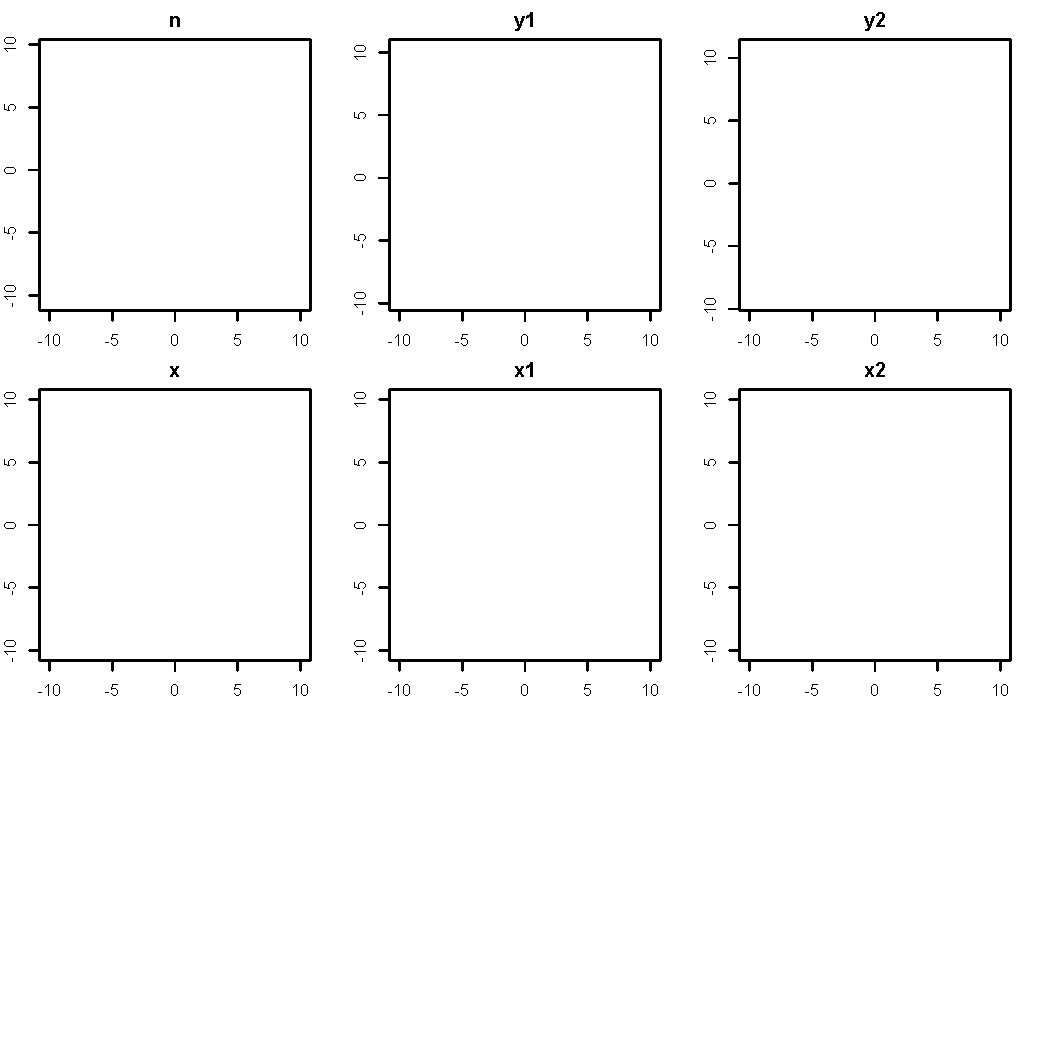
\includegraphics{scatterPlotE21.pdf}
	\caption{Scatter plots of the data.} \label{fig:scatterE21}
\end{figure}

\subsection{Exercise 2}
The whitening matrices were:
\begin{verbatim}
> whiteningY1
           PC1        PC2
[1,] 0.1695626  0.2945006
[2,] 0.8716748 -0.5018783
> whiteningY2
          PC1        PC2
[1,] 0.170350  0.2939907
[2,] 0.870344 -0.5043123
> whiteningX1
           PC1        PC2
[1,] 0.1639257  0.2850347
[2,] 0.8680057 -0.4991970
> whiteningX2
            PC1        PC2
[1,] -0.1635482 -0.2860464
[2,] -0.8673773  0.4959264
\end{verbatim}
PCA:
\begin{verbatim}
> prcomp(y1)
Standard deviations:
[1] 2.9426781 0.9942015

Rotation:
           PC1        PC2
[1,] 0.4989681  0.8666204
[2,] 0.8666204 -0.4989681
> prcomp(y2)
Standard deviations:
[1] 2.9430913 0.9941372

Rotation:
           PC1        PC2
[1,] 0.5013556  0.8652413
[2,] 0.8652413 -0.5013556
> prcomp(x1)
Standard deviations:
[1] 3.0412644 0.9986868

Rotation:
           PC1        PC2
[1,] 0.4985415  0.8668658
[2,] 0.8668658 -0.4985415
> prcomp(x2)
Standard deviations:
[1] 3.034897 1.000858

Rotation:
            PC1        PC2
[1,] -0.4963519 -0.8681214
[2,] -0.8681214  0.4963519
\end{verbatim}
\begin{figure}\centering
	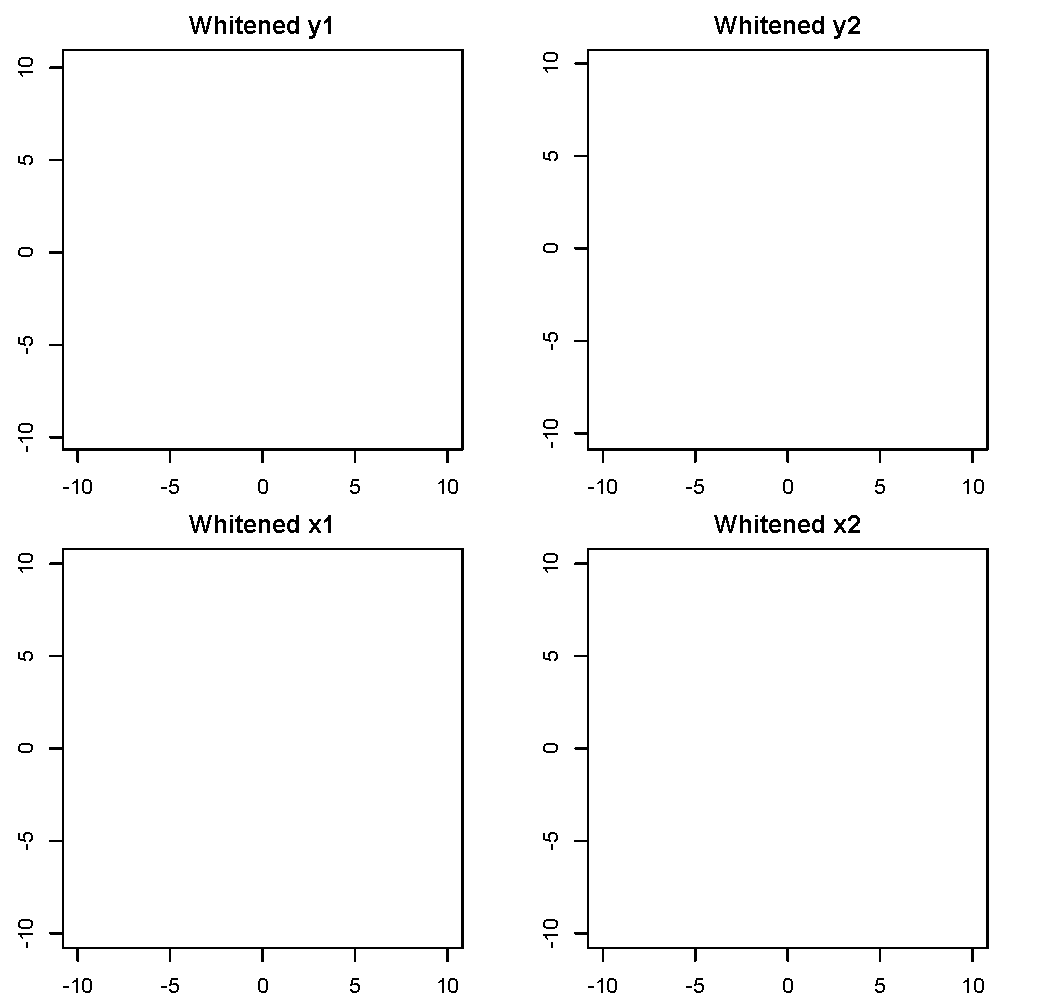
\includegraphics{scatterPlotOfWhitenedE22.pdf}
	\caption{Scatter plots of the whitened data.} \label{fig:scatterWhiteE22}
\end{figure}

\subsection{Exercise 3}
Kurtosis maximized for these alpha:
\begin{verbatim}
> maxAlphaY1
[1] 1.006316
> maxAlphaY2
[1] 0.7390133
> maxAlphaX1
[1] 0.7798949
> maxAlphaX2
[1] 0.5220264
\end{verbatim}
\begin{figure}\centering
	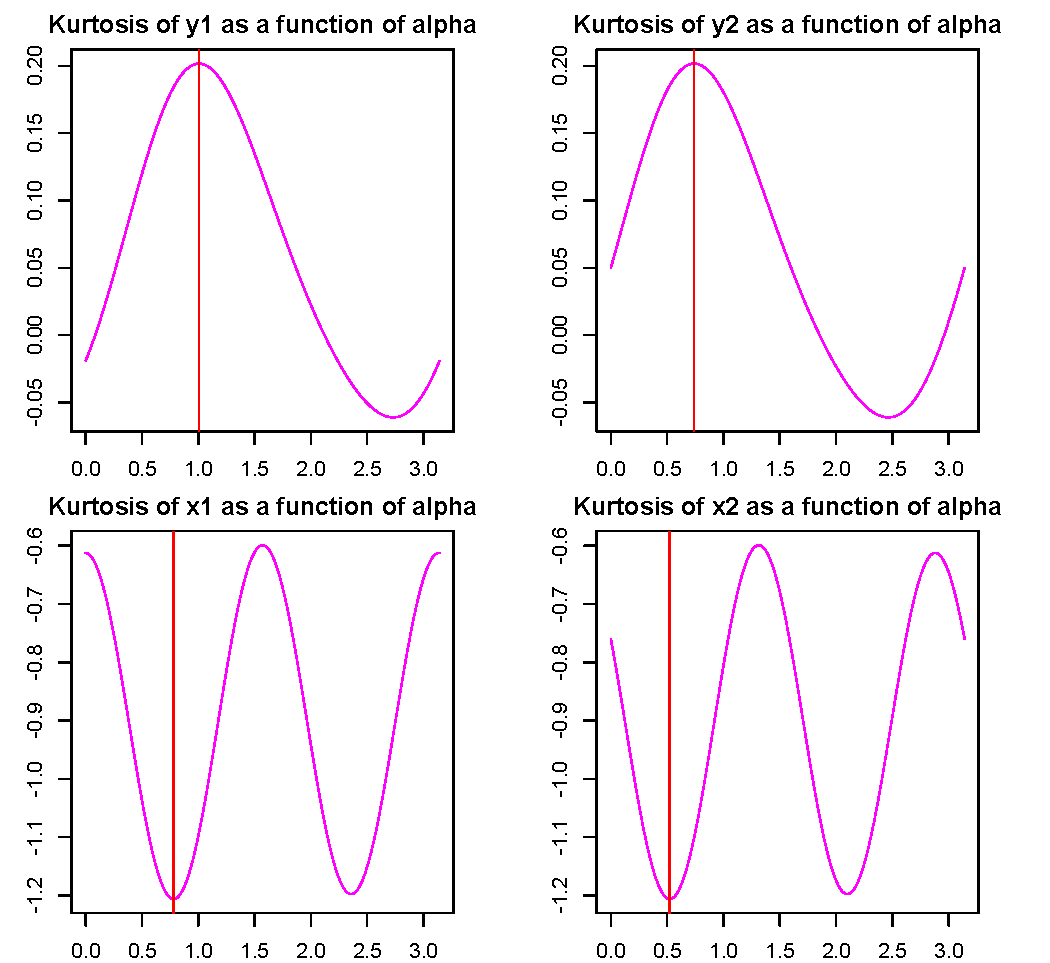
\includegraphics{kurtosisAlphaE23.pdf}
	\caption{Kurtosis as a function of alpha.} \label{fig:kurtosisAlphaE23}
\end{figure}
\subsection{Exercise 4}
\begin{verbatim}
> A1
       [,1]    [,2]
[1,] 0.4483 -1.6730
[2,] 2.1907 -1.4836
> estimatedA1forUniform
          [,1]      [,2]
[1,] 0.4586854 -1.668015
[2,] 2.1968702 -1.488719
> A2
       [,1]    [,2]
[1,] 0.0000 -1.7321
[2,] 1.7321 -2.0000
> estimatedA2forUniform
           [,1]      [,2]
[1,] 0.01227525 -1.724465
[2,] 1.74334166 -1.999660

\end{verbatim}
\subsection{Exercise 5}

\end{document}
